\documentclass[11pt]{article}            % Report class in 11 points
\parindent0pt  \parskip10pt             % make block paragraphs
\usepackage{graphicx}
\usepackage{listings}
\usepackage[document]{ragged2e}
\usepackage{float}
\newcommand\tab[1][1cm]{\hspace*{#1}}
\graphicspath{ {images/} }
\usepackage{graphicx} %  graphics header file
\begin{document}
\begin{titlepage}
    \centering
  \vfill
    
\includegraphics[width=8cm]{uni_logo.png} \\ 
	\vskip2cm
    {\bfseries\Large
	Data Structures  \& Algorithms \\ (CS09203)\\
	
	\vskip2cm
	Lab Report 
	 
	\vskip2cm
	}    

\begin{center}
\begin{tabular}{ l l  } 

Name: & Muhammad Umer \\ 
Registration \#: & CSU-F16-104 \\ 
Lab Report \#: & 07 \\ 
 Dated:& 21-05-2018\\ 
Submitted To:& Mr. Usman Ahmed\\ 

 %\hline
\end{tabular}
\end{center}
    \vfill
    The University of Lahore, Islamabad Campus\\
Department of Computer Science \& Information Technology
\end{titlepage}


    
    {\bfseries\Large
\centering
	Experiment \# 1 \\

Create a C++ program to implement the graph and add edges in the adjacency list and display added edges.\\
	
	}    
 \vskip1cm
 \textbf {Objective}\\  To understand and implement the graph with basic edges insertion in the adjacency list.
 
 \textbf {Software Tool} \\
1. Sublime Text Editor\\
2. Dev C++\\
3. Window 7 (32 Bit)\\

\section{Theory }              
\justify Graph is a data structure that consists of following two components:\\~\\
1. A finite set of vertices also called as nodes.\\
2. A finite set of ordered pair of the form (u, v) called as edge. The pair is ordered because (u, v) is not same as (v, u) in case of directed graph(di-graph). The pair of form (u, v) indicates that there is an edge from vertex u to vertex v. The edges may contain weight/value/cost.\\~\\
Graphs are used to represent many real life applications: Graphs are used to represent networks. The networks may include paths in a city or telephone network or circuit network. Graphs are also used in social networks like linkedIn, facebook. For example, in facebook, each person is represented with a vertex(or node). Each node is a structure and contains information like person id, name, gender and locale.\\~\\
Following is an example undirected graph with 5 vertices.\\~\\
\begin{figure}[H]
\centering
  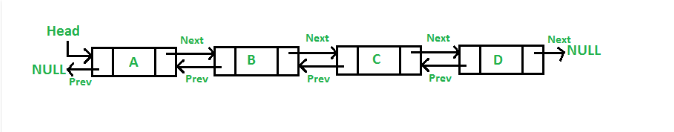
\includegraphics[width=12cm,height=6cm,keepaspectratio]{5.png}    
\end{figure}
\section{Task}  
\subsection{Procedure: Task 1 Inserting Edges}
The following code is the representation of the above graph using STL
\begin{lstlisting}[language=C++]
void addEdge(vector<int> adj[], int u, int v)
{
	adj[u].push_back(v);
	adj[v].push_back(u);
}
\end{lstlisting}

\subsection{Procedure: Task 2 Displaying the Edges}     
\begin{lstlisting}[language=C++]
void printGraph(vector<int> adj[], int V)
{
	for (int v = 0; v < V; ++v)
	{
		cout << "\n Adjacency list of vertex "
			<< v << "\n head ";
		for (auto x : adj[v])
		cout << " -> " << x;
		printf("\n");
	}
}
\end{lstlisting}

\subsection{Procedure: Task 3 Main Function}     
\begin{lstlisting}[language=C++]
#include<bits/stdc++.h>
using namespace std;

int main()
{
	int V = 5;
	vector<int> adj[V];
	addEdge(adj, 0, 1);
	addEdge(adj, 0, 4);
	addEdge(adj, 1, 2);
	addEdge(adj, 1, 3);
	addEdge(adj, 1, 4);
	addEdge(adj, 2, 3);
	addEdge(adj, 3, 4);
	printGraph(adj, V);
	return 0;
}

Output:
\end{lstlisting}
Consider the Figure 1 (in the end of this document) for the output of the above graph.\\~\\
Note: My IDE (Dev C++) doesn't support C++11, as the above code is written in C++11, I run this code in the online IDE "https://ide.geeksforgeeks.org/index.php", which give me the output showed in Figure 1

\textbf{Source Code} \\
https://goo.gl/ccBvqK

\begin{figure}[b!]
\centering
  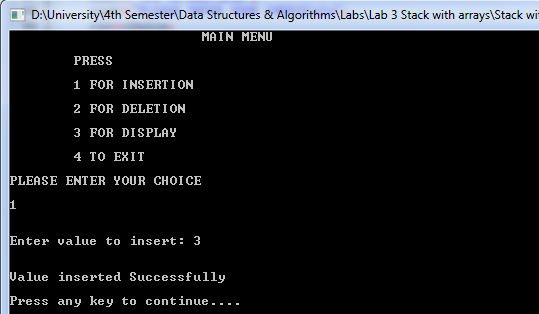
\includegraphics[width=12cm,height=6cm,keepaspectratio]{1.png}
\caption{Adjacency list representation of the graph}
\label{Figure:1}    
\end{figure}

\section{Conclusion}
\justify Graphs are used to represent many real life applications: Graphs are used to represent networks. The networks may include paths in a city or telephone network or circuit network. Graphs are also used in social networks like linkedIn, facebook. For example, in facebook, each person is represented with a vertex(or node). Each node is a structure and contains information like person id, name, gender and locale.\\~\\

\tab[6cm] \noindent\rule{6cm}{0.4pt}\\
\tab[6cm] (Concerned Teacher/Lab Engineer)


 
\end{document}                          % The required last line
